\chapter[SCP-023 黑煞星]{
    SCP-023 Black Shuck\\
    SCP-023 黑煞星
}

\label{chap:SCP-023}

\begin{figure}[H]
    \centering
    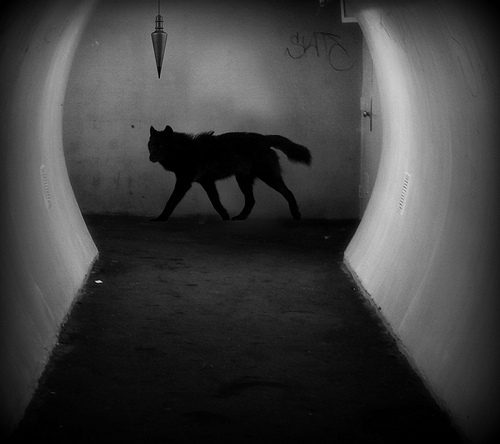
\includegraphics[width=0.5\linewidth]{images/SCP.023.jpg}
    \caption*{SCP-023於SCP-███逃脫事件中收容於暫時收容區}
\end{figure}

\bb{項目編號:}SCP-023

\bb{項目等級:}Euclid

\bb{特殊收容措施:}\dd{SCP-023應收容於一間5X5米的標準收容單位內。} SCP-023收容於Site-██的一處收容區,該區結構為兩道迴廊交錯構成的叉狀建物,並延邊緣圍起圍牆; 四端任一走道的長度皆長於3米,且參號及肆號迴廊端點除了正常的門外,也附加了假門。監視攝影機設於四端端點的門上方。

不論何時,SCP-023的兩個眼窩應以硬橡膠制的球狀眼部植入物填充。當植入物有劣化的情形時,必須進行更換。劣化情形可依在監視平台觀察到的"火光"亮度來判別。當亮度超過██燭光時,必須於12小時內更換植入物。更換時應注意,只能在完全日落後進行更換,且不可同時更換兩側的植入物。任何人員不可在任何時間直視SCP-023的眼窩內部。

依據\hyperref[chap:DOC-incident-023-27]{事件報告023-27},所有具有反光面的物品,如顯示器,螢幕,或任何一種眼鏡,皆不允許出現在SCP-023的收容區半徑30米內。上述要求亦包括連線至監視攝影機的螢幕零部件。於收容區外定點哨點的保安人員亦強制遵行上述要求。

關於SCP-023的相關試驗皆已無限期推延。

\bb{描述:}SCP-023是一隻大型無性別的黑色長毛犬科生物(肩高1.5米),\dd{有一對亮橘紅色的\mbox{\hyperref[chap:TAIL-mothers-love]{眼睛}}跟一口突出的牙齒}(見\hyperref[chap:DOC-incident-report-023-26]{事件報告023-26})。 當一位個體與SCP-023發生視線接觸時,自視線錯開起約1年內,該個體或個體的近親親屬之一將會死亡。盡管更進一步的試驗皆已無限期推延,但依據當前資料,個體死亡的機率會比個體的親屬高,且受害者之間沒有明顯的特殊相關性,也沒有發現有特別偏向某類受害者的情形。這可能表示SCP-023的受害者是完全隨機的, 然而無法得知之前試驗資料的受害者是死於1年期間的初期或是末期。試圖在1年末期前,處決所有有過與SCP-023視線接觸的個體及其親屬們的行動,因[資料刪除]而結束。

SCP-023的受害者經驗屍後發現,他們的外觀毫無受傷痕跡,然而其餘部份已被經高度壓縮過的灰燼“填滿”;其餘部份包括但不限於任何器官組織及循環系統。所有受害人的肌肉組織,骨骼及腦組織皆有暴露於攝氏██度以上的跡象。

SCP-023如被收容於外觀不是近似於“十字路口”的設施時,牠將能傳躍出牆外,到達最近距離且符合收容條件的地區,並焚化路徑上所有物質。

基金會首次注意到SCP-023是在███████的一座教堂,當時牠在集會中發起一次攻擊,直接殺害 █位平民,並因視線接觸而[已刪節]。於回收SCP-023後,所有證人及倖存者皆施以B級記憶清除。該次事故已掩飾為縱火案件。

\bb{附錄023-001}\\
在██\slash ██\slash ████,SCP-023穿牆脫出收容區(事故報告023-01)。之後於Site-███內兩道迴廊的交叉口發現。特工█████ 注意到SCP-023看起來很像[已刪節]。SCP-023的特殊收容措施已更新。研究助理███████因此次過失受到申誡。

\bb{附錄023-002}\\
自10\slash 12\slash ██94第一次收容以來,已有 ███ 位工作人員及██位平民的死亡歸因於SCP-023。

\bb{附錄023-003:}\\
正在評估升至Keter的請求。

\bb{附錄023-004:}\\\hyperref[chap:SCP-1111]{SCP-1111-1}和SCP-023可能是同一现象的两个变体,因为它们被发现具有几个相同的特性:对地理位置的敏感性、具有破坏性、类似的犬类外观。对这一现象的深入调查正在进行中。由于SCP-1111-1无法捕获,研究目前集中在SCP-023上。
